\section{Data Processing Pipeline}

\subsection{Predicting CO\textsubscript{2} Emissions 2020}
\subsubsection{Motivation}
One of the major problems was to find emission data. Our EDGAR dataset ends in 2018. The goal of this part is to predict the emissions for the two next years 2019 and 2020 in the case that the COVID crisis didn't occur. The first idea was to find any relationship between the countries \co emissions and the different activities sector such as industry, mobility, international aviation etc.
The problem we encountered was that these data were not temporally overlapping. As mentioned before, our EDGAR emissions dataset ends in 2018 and the samples are yearly. Furthermore, our mobility and aviation data is daily and starting from January 2020. No relationship can be found if the data are not temporally crossing. The second idea was to predict these emissions for 2019 and 2020 from its evolution since 1970 .
\subsubsection{Predicted Country CO\textsubscript{2} Emissions without Considering COVID-19}
\paragraph*{Polynomial regression}
In order to predict the emissions for each country for the two next years starting from 2018 we need a model that describes the \co emissions evolution. A model based on regression learning is used. The first two questions arising are  which model to use and what the parameters of such a model should be.
Choosing between a linear and a polynomial model is evident. The evolution of \co is for many countries is too complex and a linear model does not offer enough precision to describe such curves.
The easiest curve to learn has is Bangladesh, shwowing an approximately exponential shape, which can be easily expressed with a polynomial. But there are complexer shapes where the emissions increase is not stable.
\begin{figure}[h!]
	\centering
	\subfloat[Bangladesh]{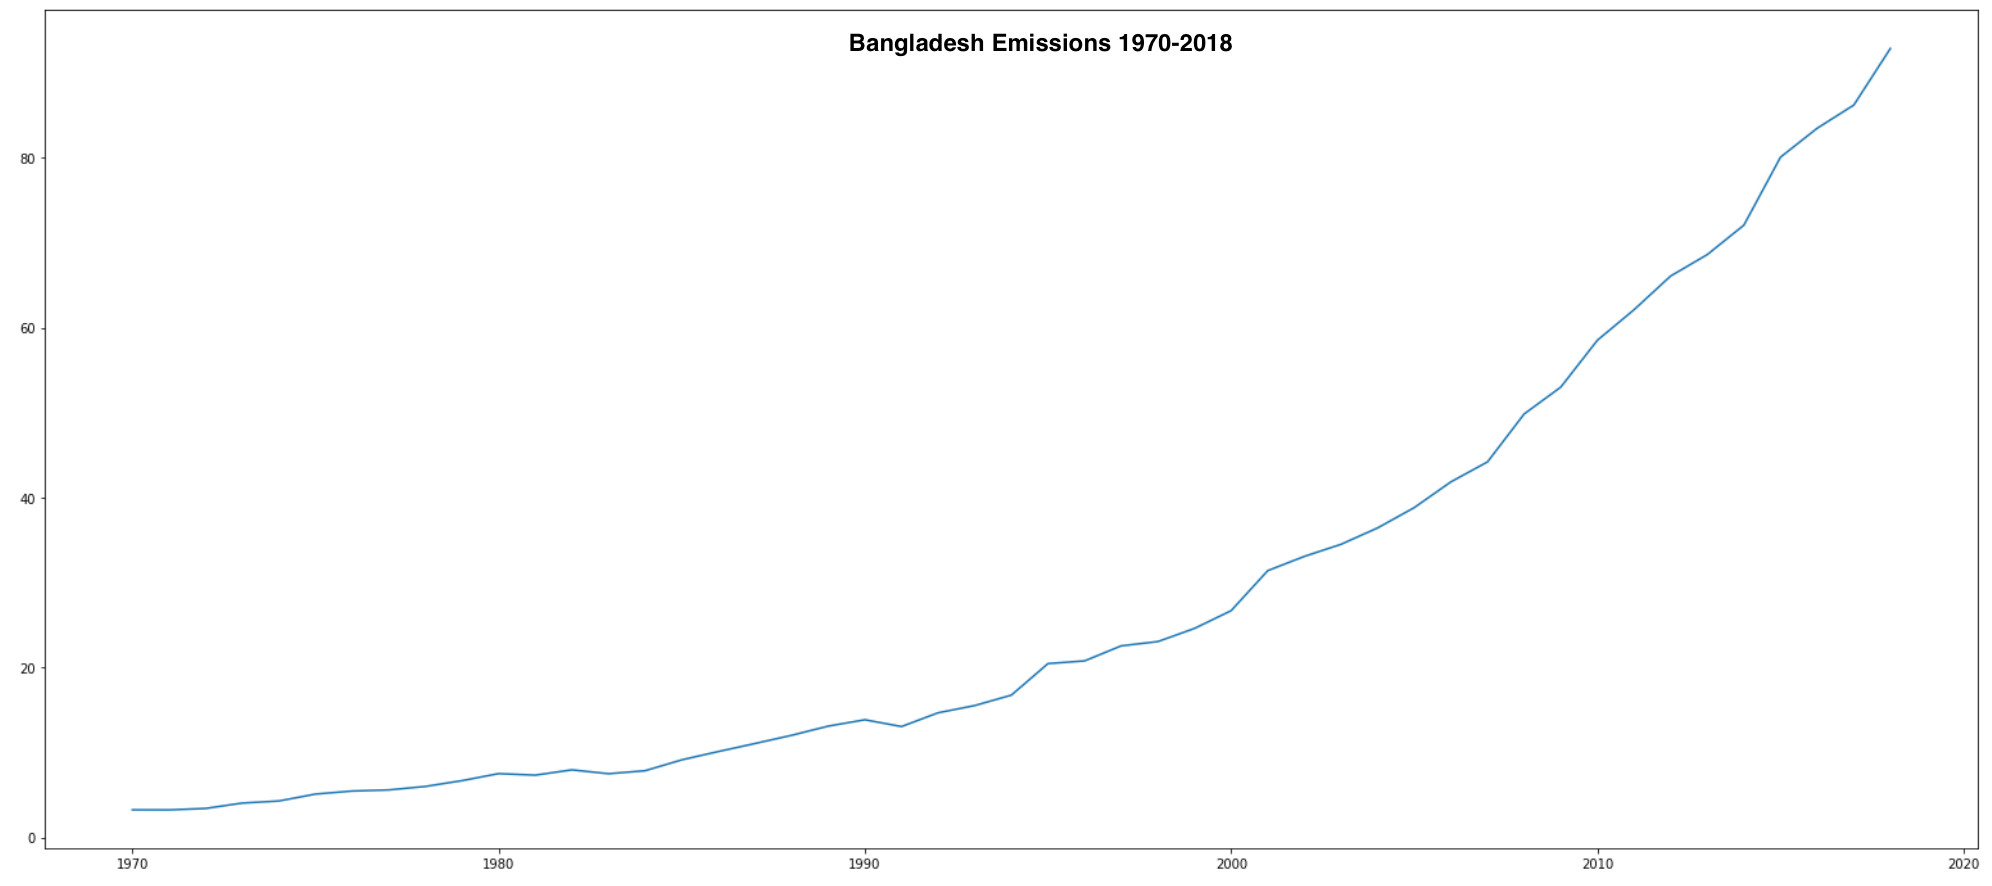
\includegraphics[width=0.5\linewidth]{ziedPNGS/Bangladesh}}
	\subfloat[Ireland]{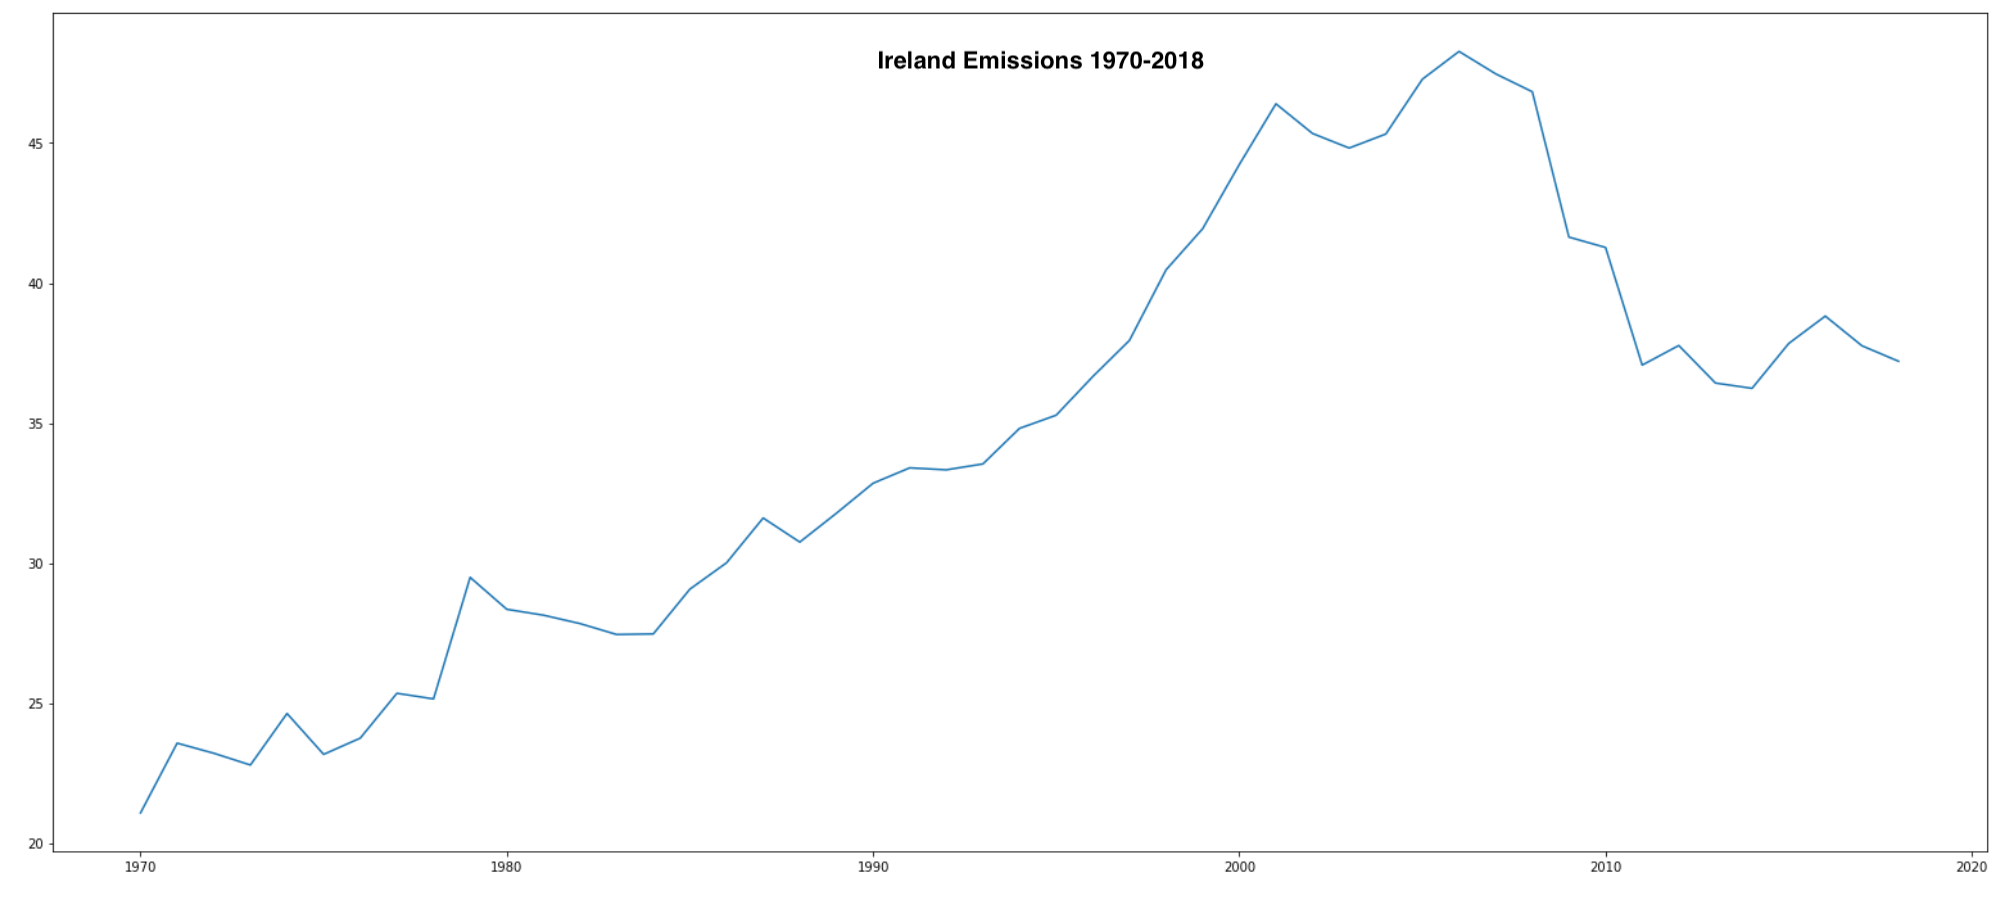
\includegraphics[width=0.5\linewidth]{ziedPNGS/Ireland}}
	\caption{Example of a stable and unstable emissions evolution.}
	\label{fig:Emissions}
\end{figure}
\newline
For choosing the size $k$ of a polynomial $\sum_{n=1}^{k}{a_n*x^n}$, fifteen models of size $k=[1,\dots,15]$ were trained and the results were compared to the real data using the root-mean-sqaure (RMS) in \autoref{fig:RMS}.
\begin{figure}[h!]
	\centering
	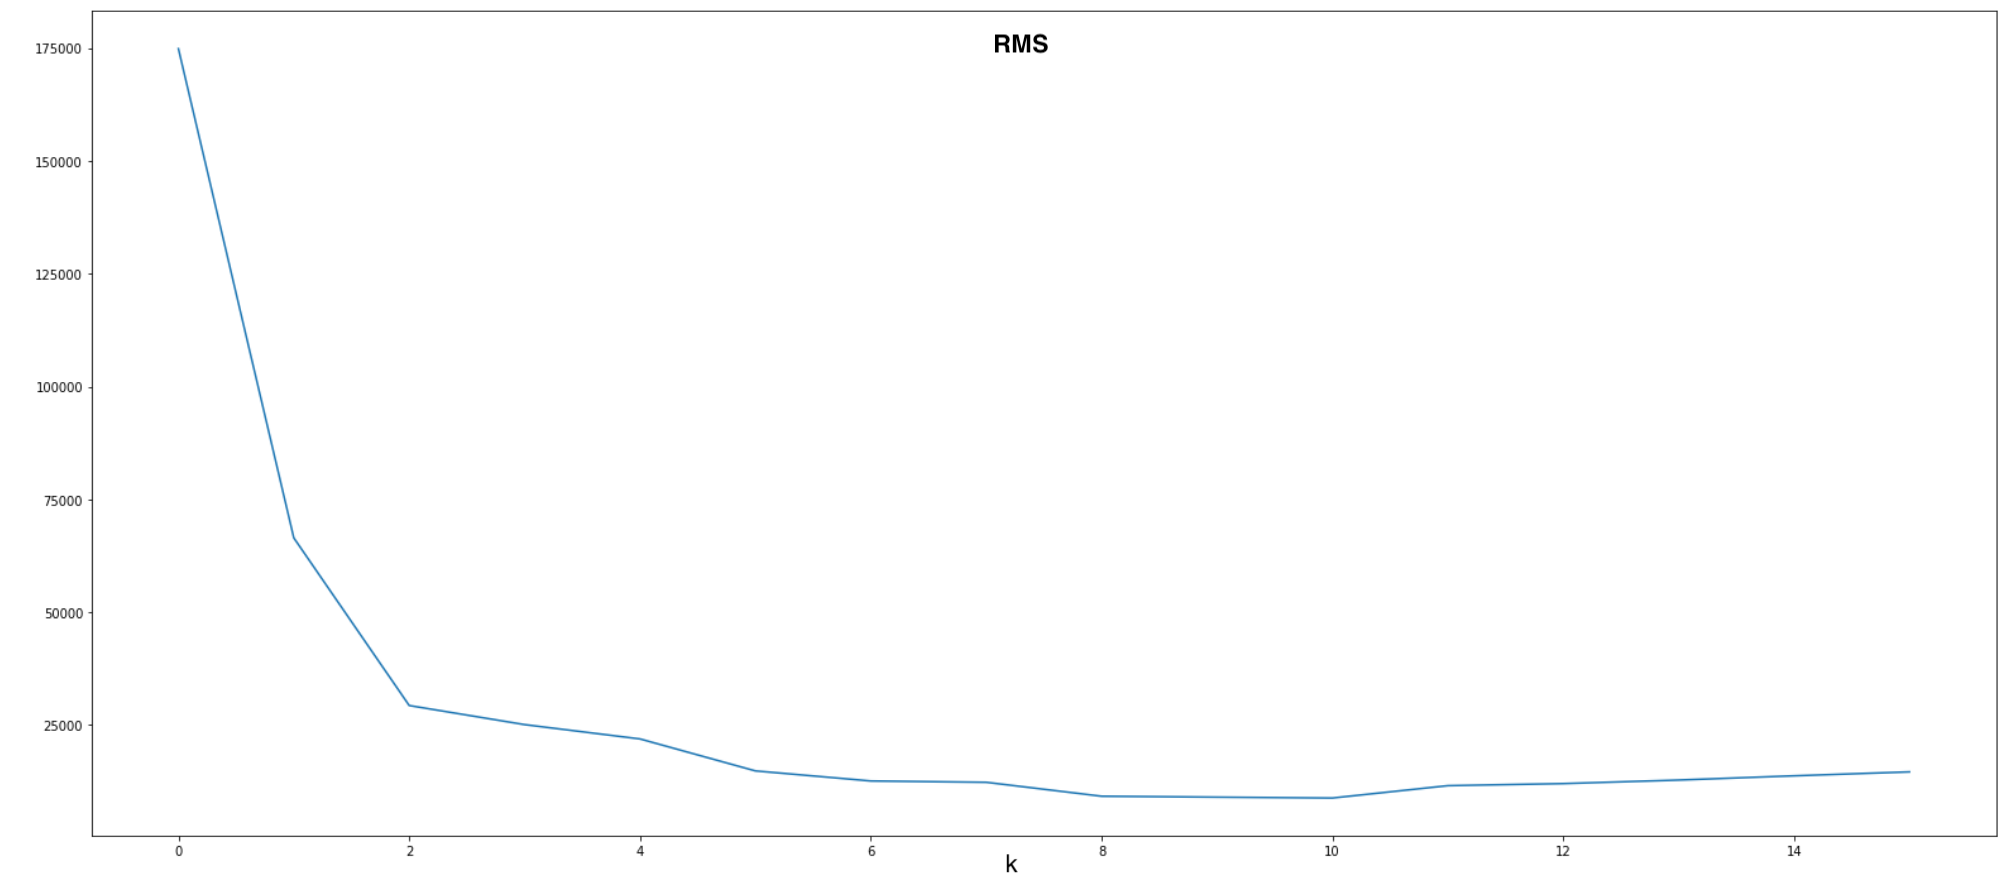
\includegraphics[width=0.7\linewidth]{ziedPNGS/RMS}
	\caption{$k=9$ delivers the smallest error.}
	\label{fig:RMS}
\end{figure}

\paragraph*{Polynomial regression's limitations}
After training a regression model for each country, the polynomials showed some plausible predictions but also many predictions where the curve has a steep drop for 2019 and 2020 \autoref{fig:firstPrediction}. The next step is to manage finding a plausible prediction for each of the eight important regions mentioned before.

\begin{figure}[h!]
	\centering
	\subfloat[Africa]{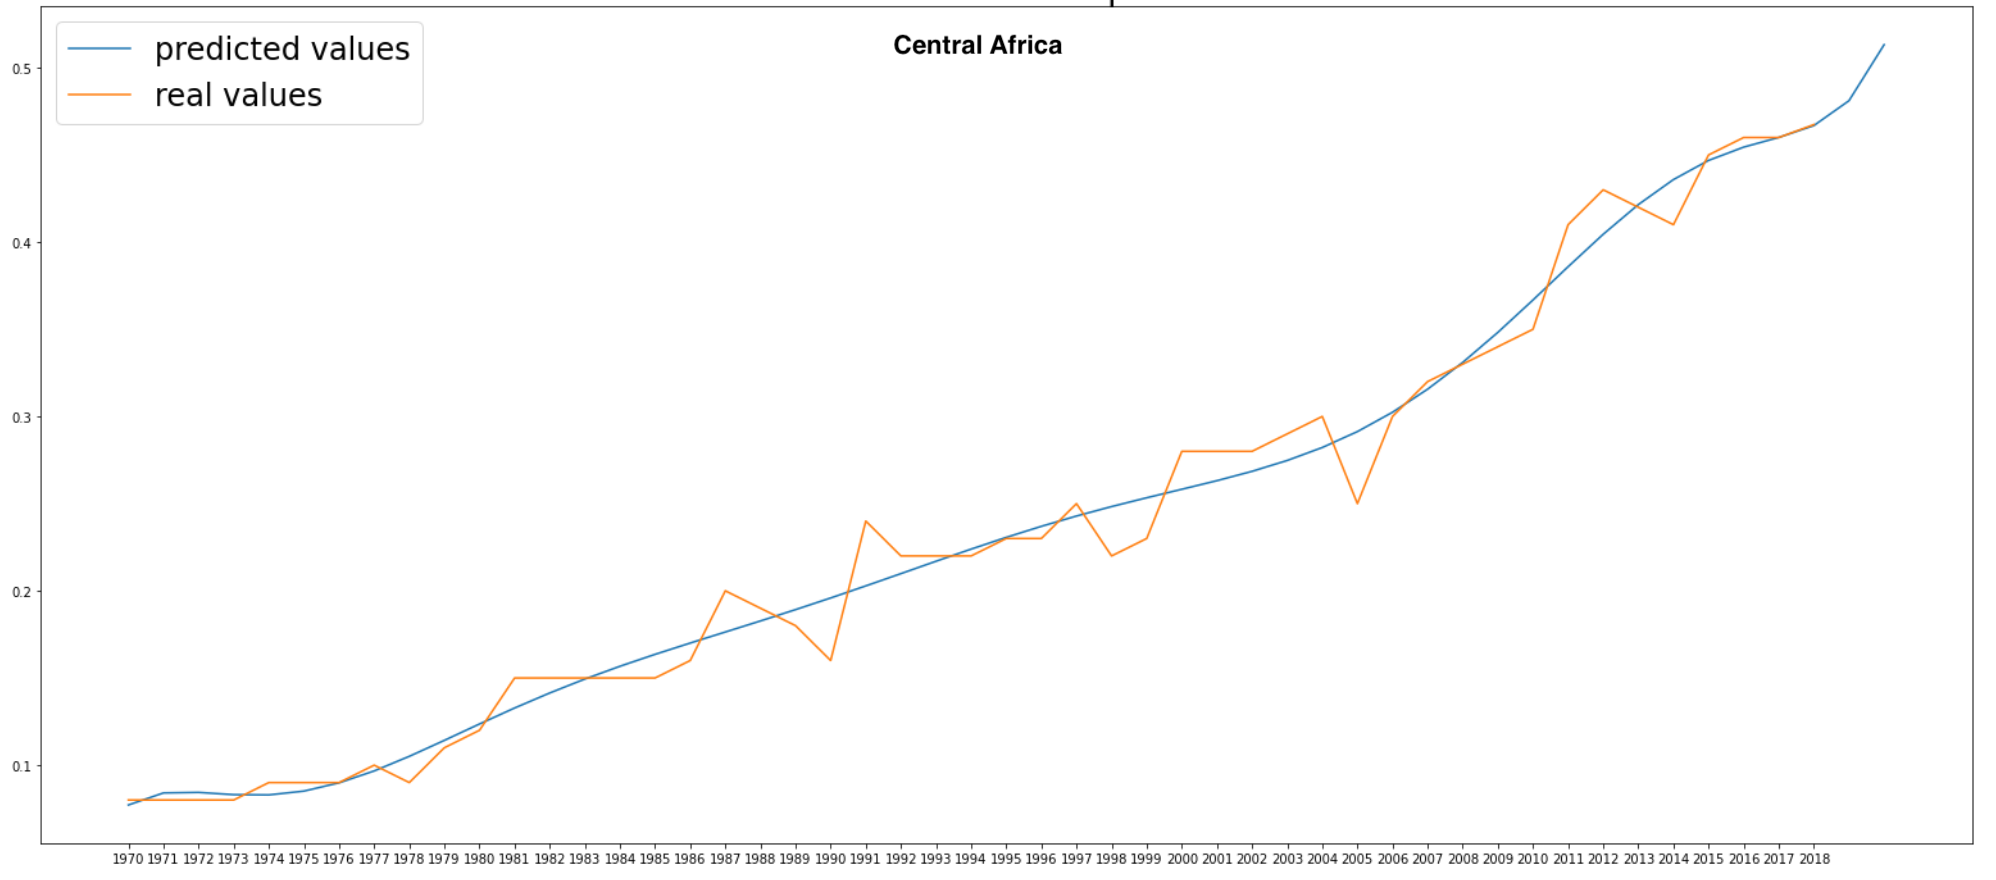
\includegraphics[width=0.5\linewidth]{ziedPNGS/Africa}}
	\subfloat[Chad]{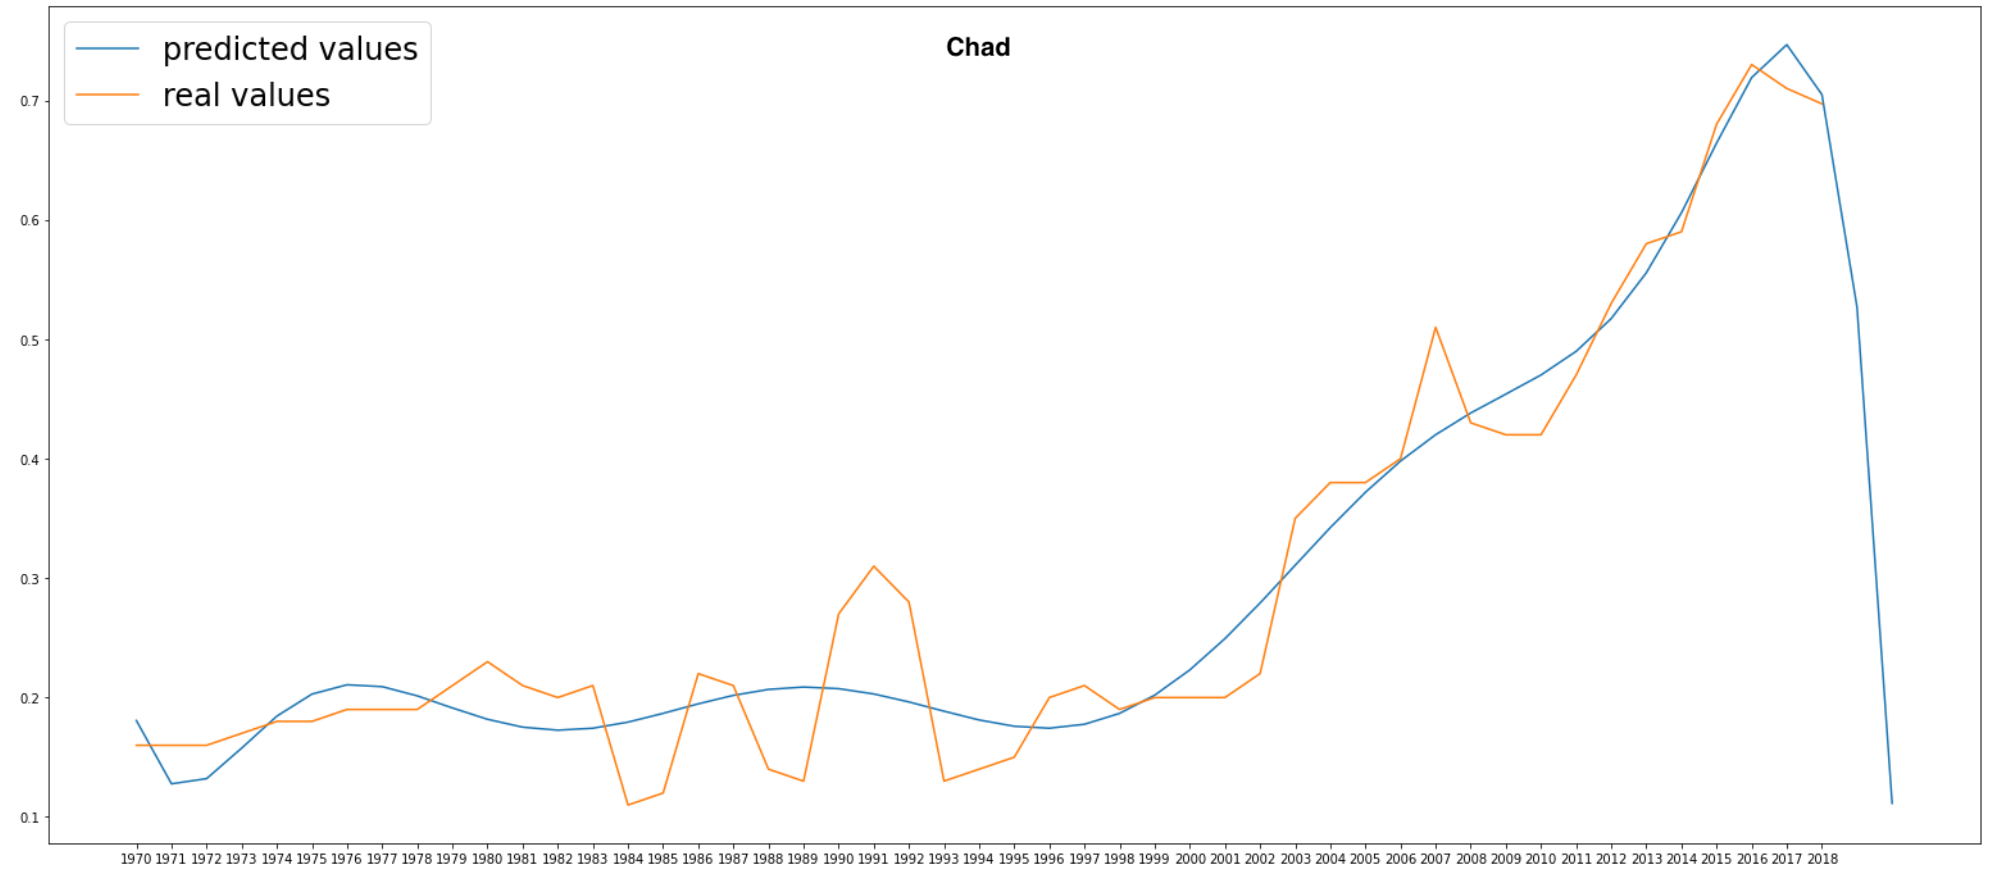
\includegraphics[width=0.5\linewidth]{ziedPNGS/Chad}}
	\caption{Example of a plausible and a wrong prediction}
	\label{fig:firstPrediction}
\end{figure}

\paragraph*{Correlation's predictions}
Looking closer to the EDGAR dataset, we can notice that some countries emissions are correlating. This make sense since the industry and a more resource-intensive way of life becomes more and more global. Using this assumption, one can take advantage of these correlations to correct the wrong predictions from our models.
Using the first prediction, we manually select the best results and look for countries with correlating emissions.
The first step is to choose the best predictions from our results. In our case we have 21 plausibly predicted values for 2019 and 2020. Having this list of countries we calculate the correlation of the real data from 1970 to 2018 of these 21 countries with every other country and filter out the correlations included in the interval $[-0.9,...,0.9]$.
Now we have a list of countries which emissions in 2019 and 2020 can be predicted from the first predictions.
For each correlation, we train a linear model using the real data from 1970 until 2018 and predict the emissions of 2019 and 2020 using the appropriate model and the predicted data from 1970 to 2020.
\begin{center}
\begin{table}[h!]%todo: Pie chart?, Values add up to 109 \% sadly
	\centering
	\begin{tabular}{ll}
		\hline
		 Country's emissions to predict& Already predicted countries emission\\
		\hline
		\hline
		 Bahrain   & Australia   \\
  		 Brazil &   Australia  \\
 		 Canada & Australia \\
 		 Dominica & Australia, Burkina Faso\\
  		 Iran & Australia, Burkina Faso, Egypt, Iceland, India, Indonesia \\
		 Iraq & Burkina Faso, India, Indonesia \\
 		 Ireland & Greece \\
		 Malta & Greece \\
 		 Haiti &  Burkina Faso, Egypt \\
 		 Singapore & Australia, Egypt, Indonesia, Malaysia, Morocco \\
 		 United Kingdom & Burkina Faso, Egypt, India, Morroco, Phlippines, Turkey, United Arab Emirates \\
 		 United States& Netherlands \\
		\hline &\\
	\end{tabular}
	\caption{Some examples of dependencies for the second predictions.}%todo: source
	\label{tab:correlations}	
\end{table}	
\end{center}
Some examples of our results are shown in the \autoref{tab:correlations}. We can see that Brazil is only correlating with Australia. In this case we predict Brazil's emissions from Australia's emissions. For Iran we have more countries correlating: Australia, Burkina Faso, Egypt and other. In this case, we can generate more predictions. From these predictions we calculate the mean value, the maximum value and the minimum value to have a better approximation.
\begin{figure}[h!]
	\centering
	\subfloat[Brazil]{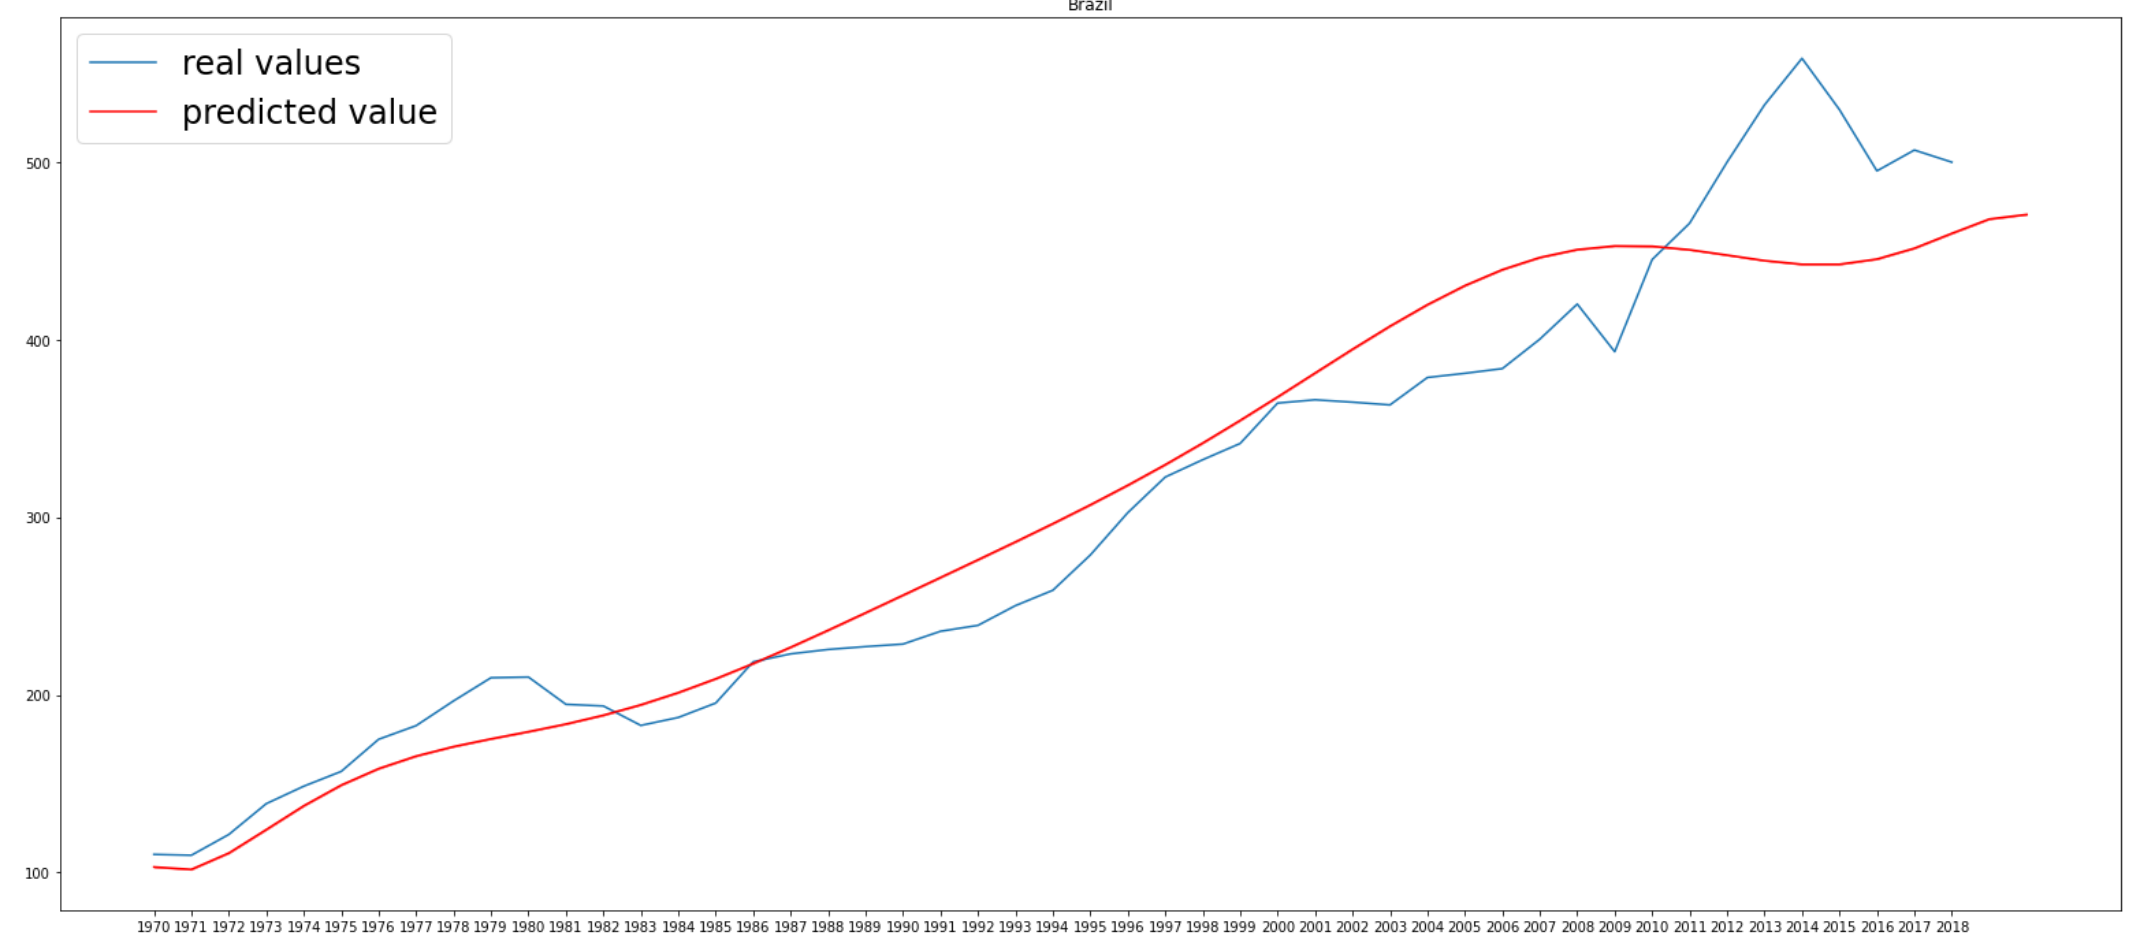
\includegraphics[width=0.5\linewidth]{ziedPNGS/Brazil}}
	\subfloat[Iran]{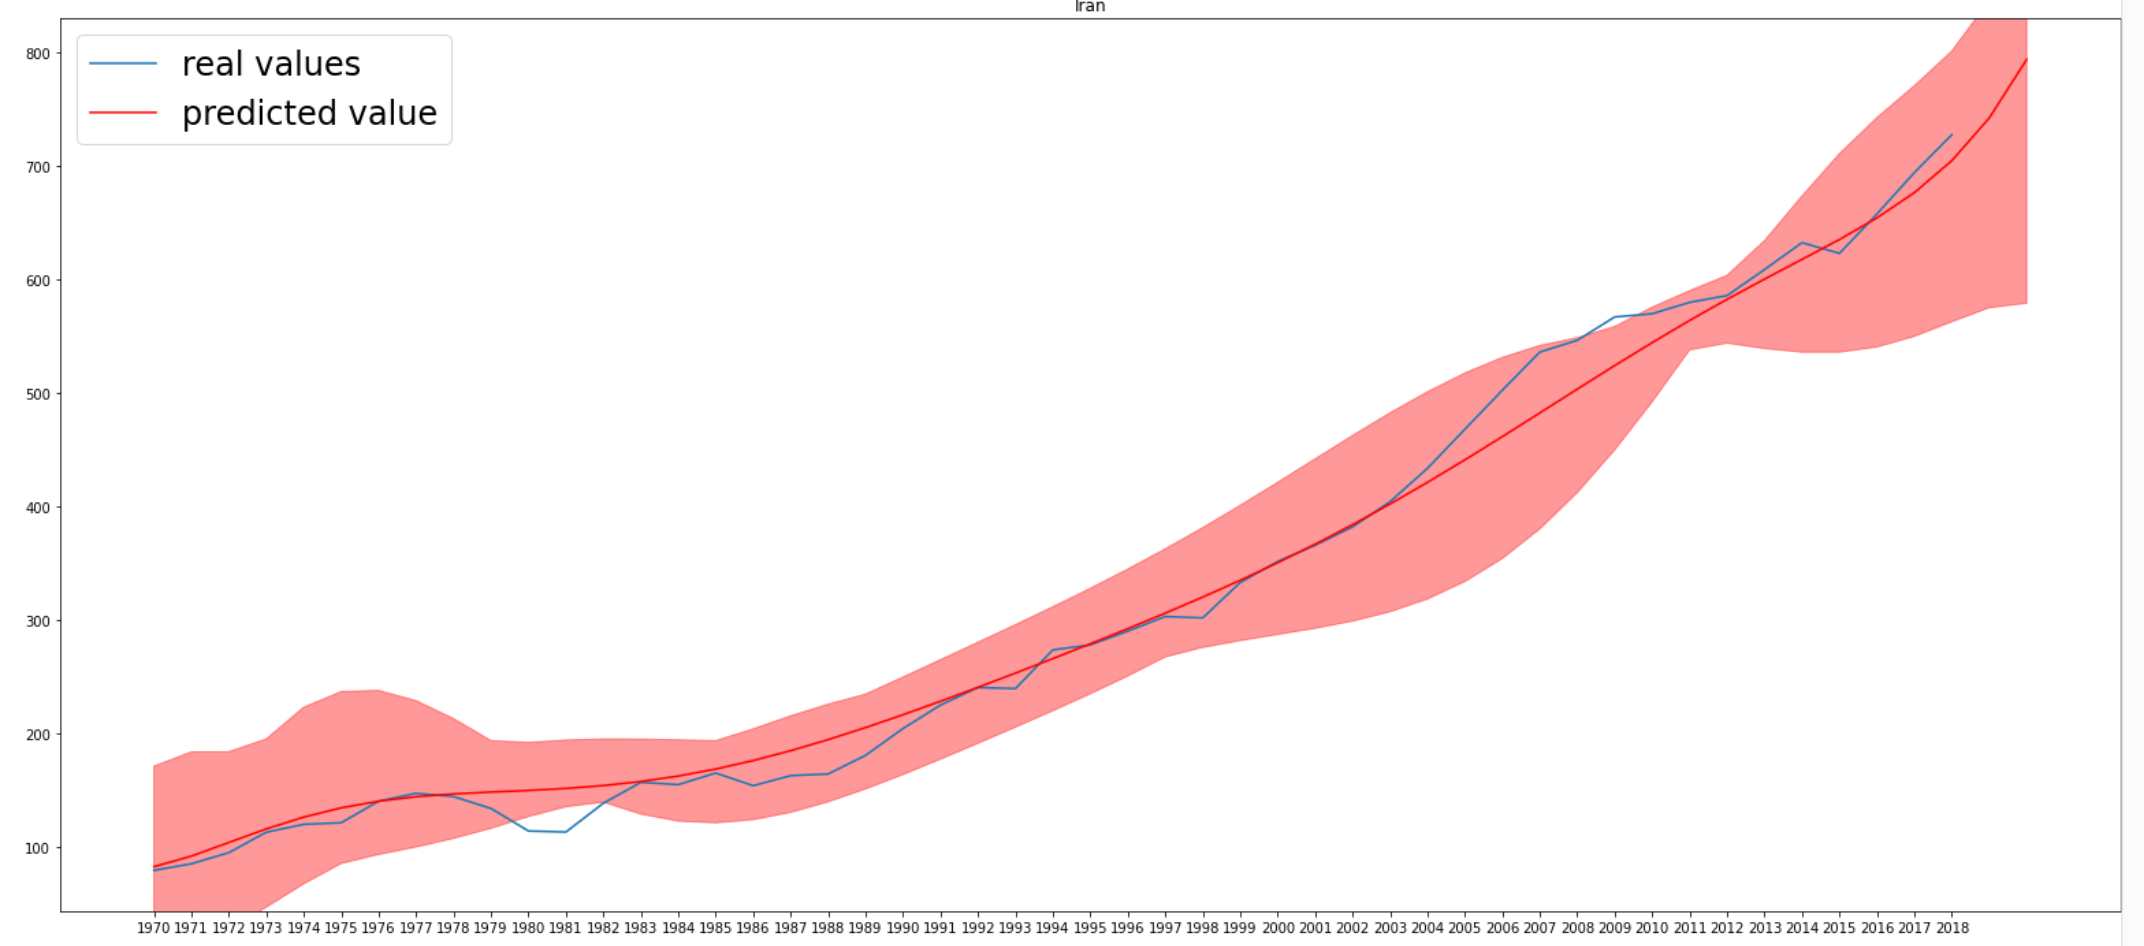
\includegraphics[width=0.5\linewidth]{ziedPNGS/Iran}}
	\caption{Brazil's emissions are predicted from Australia's emissions. Iran's emissions are predicted from the emissions of several countries.}
	\label{fig:resultsExample} % change label
\end{figure}

\subsubsection{Results and conclusion}
From the eight major countries we consider -- Canada, China, United States, Japan, Russia, Brazil, India and the EU -- India's predictions could be generated with the first prediction and the remaining countries were generated with the second predictions.
Only Russia's predictions are not available, because no correlation with any other country was found.

\begin{figure}[hbt!]
	\centering
	\subfloat[Brazil]{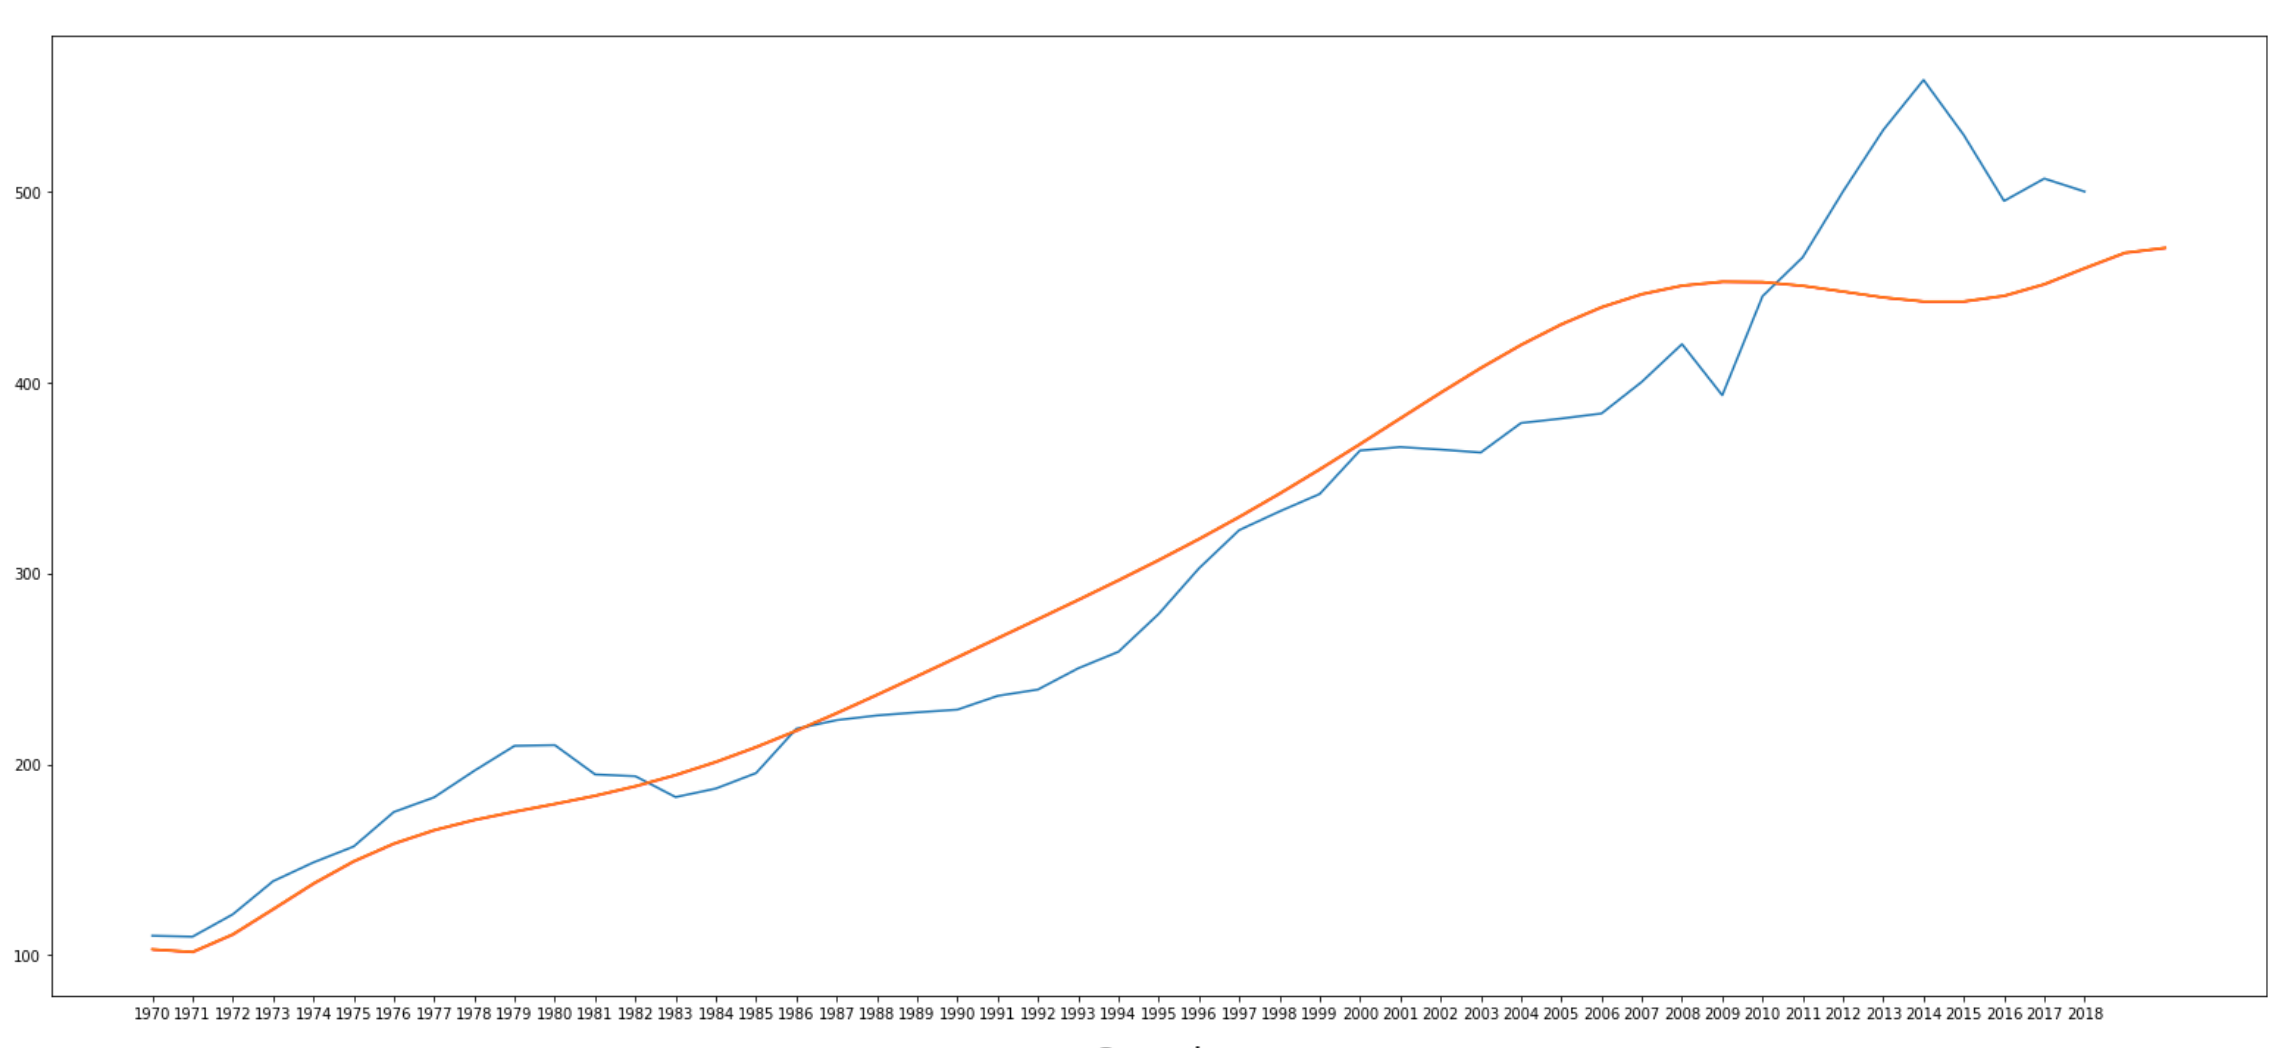
\includegraphics[width=0.5\linewidth]{ziedPNGS/br}}
	\subfloat[Canada]{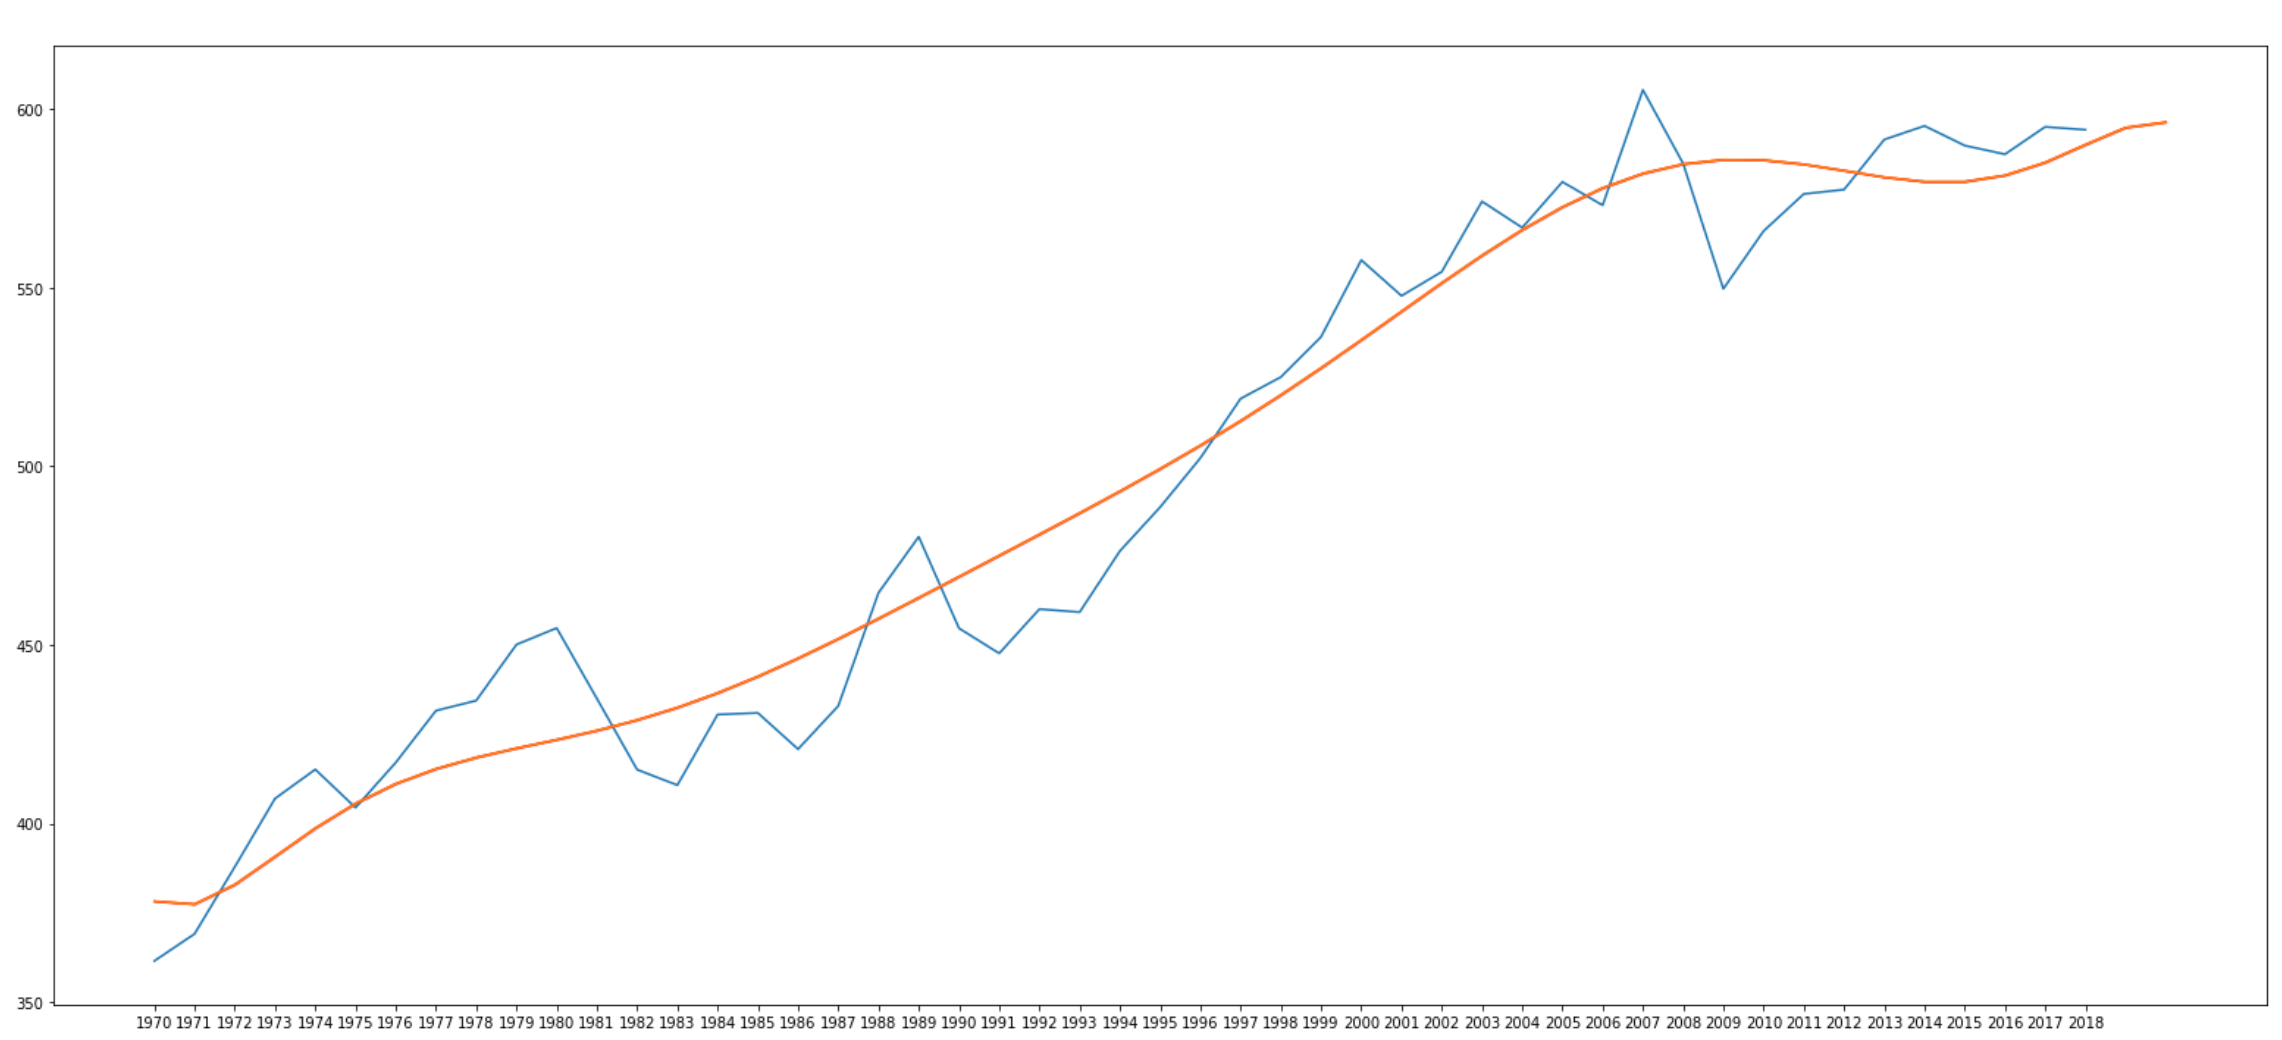
\includegraphics[width=0.5\linewidth]{ziedPNGS/2}}
	
	\subfloat[Japan]{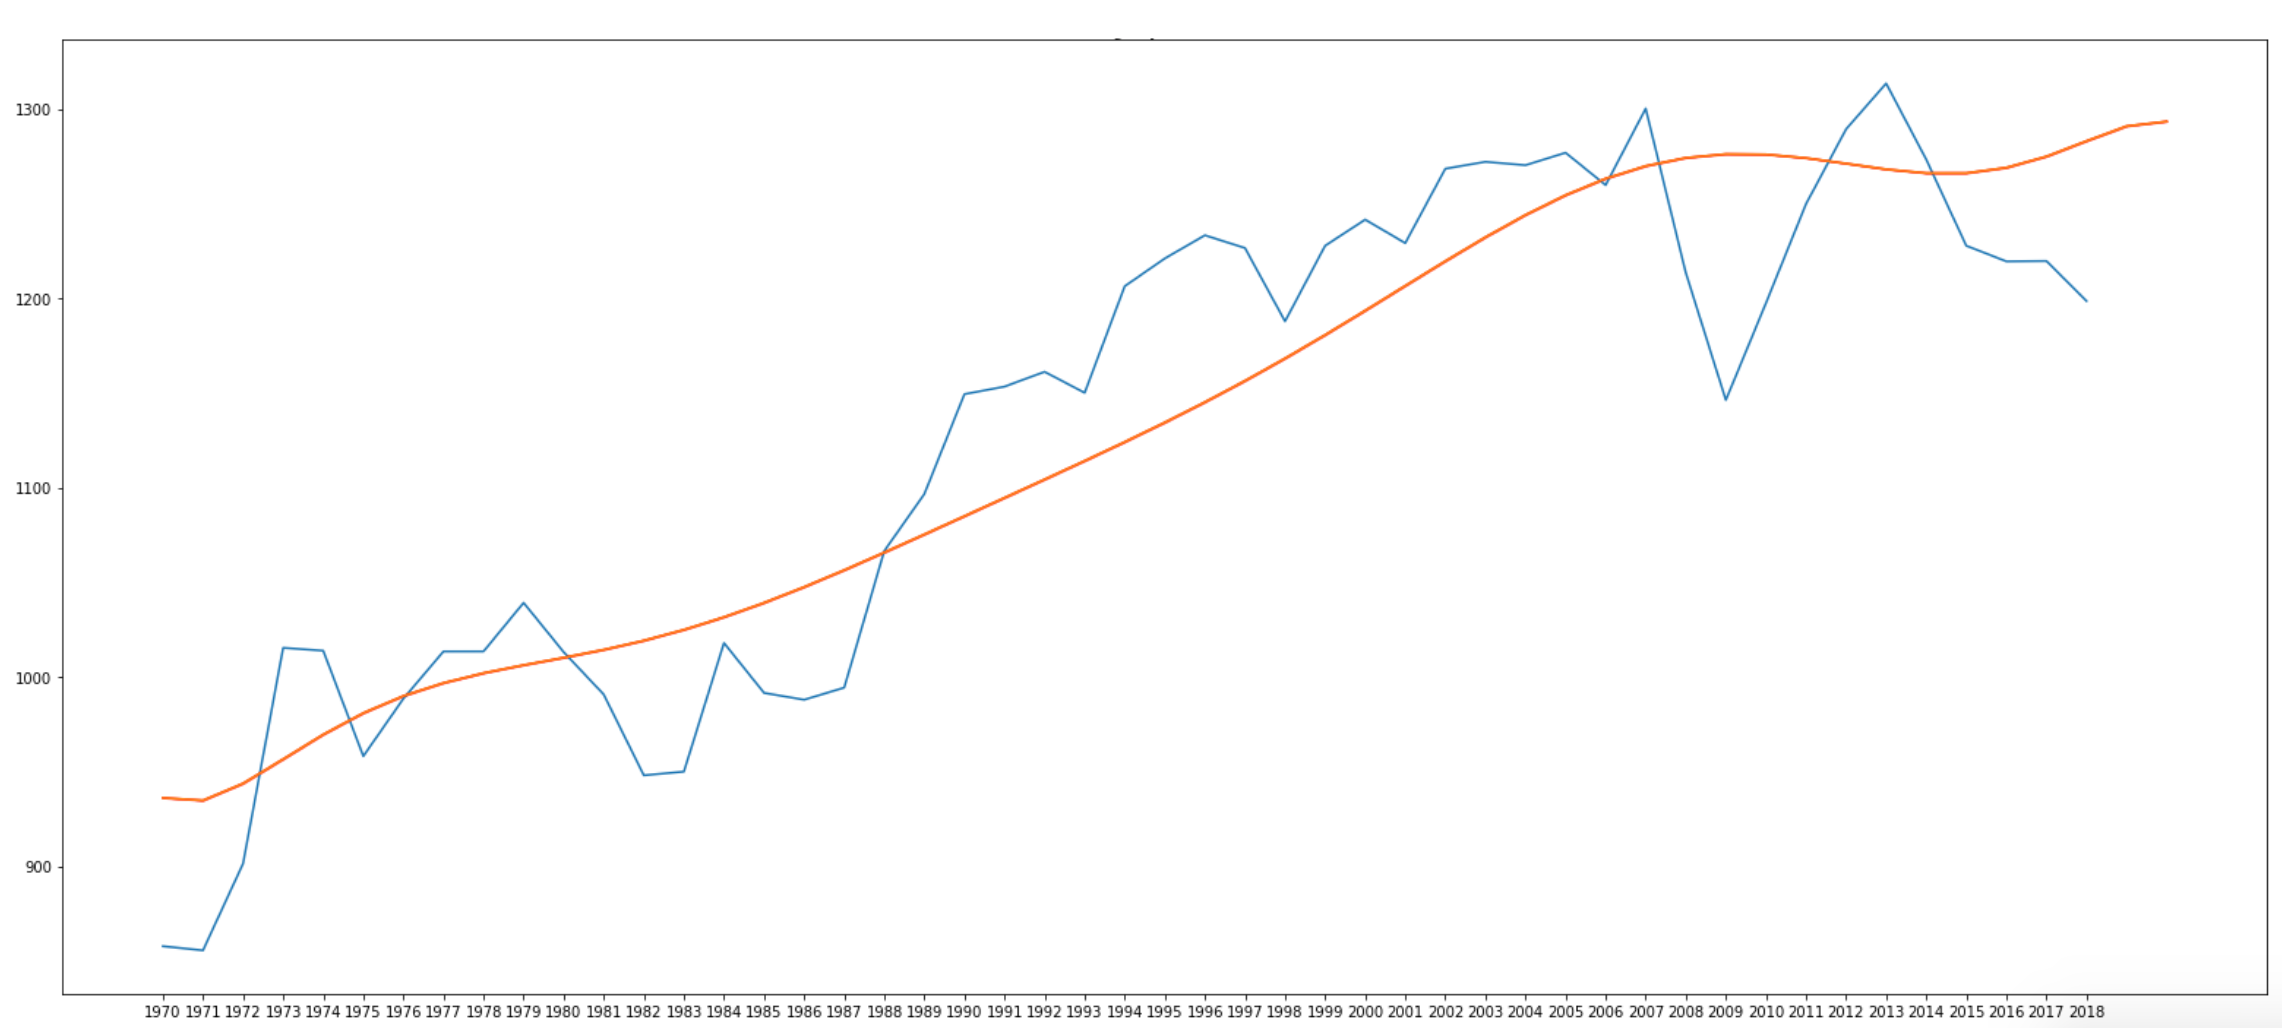
\includegraphics[width=0.5\linewidth]{ziedPNGS/3}}
	\subfloat[China]{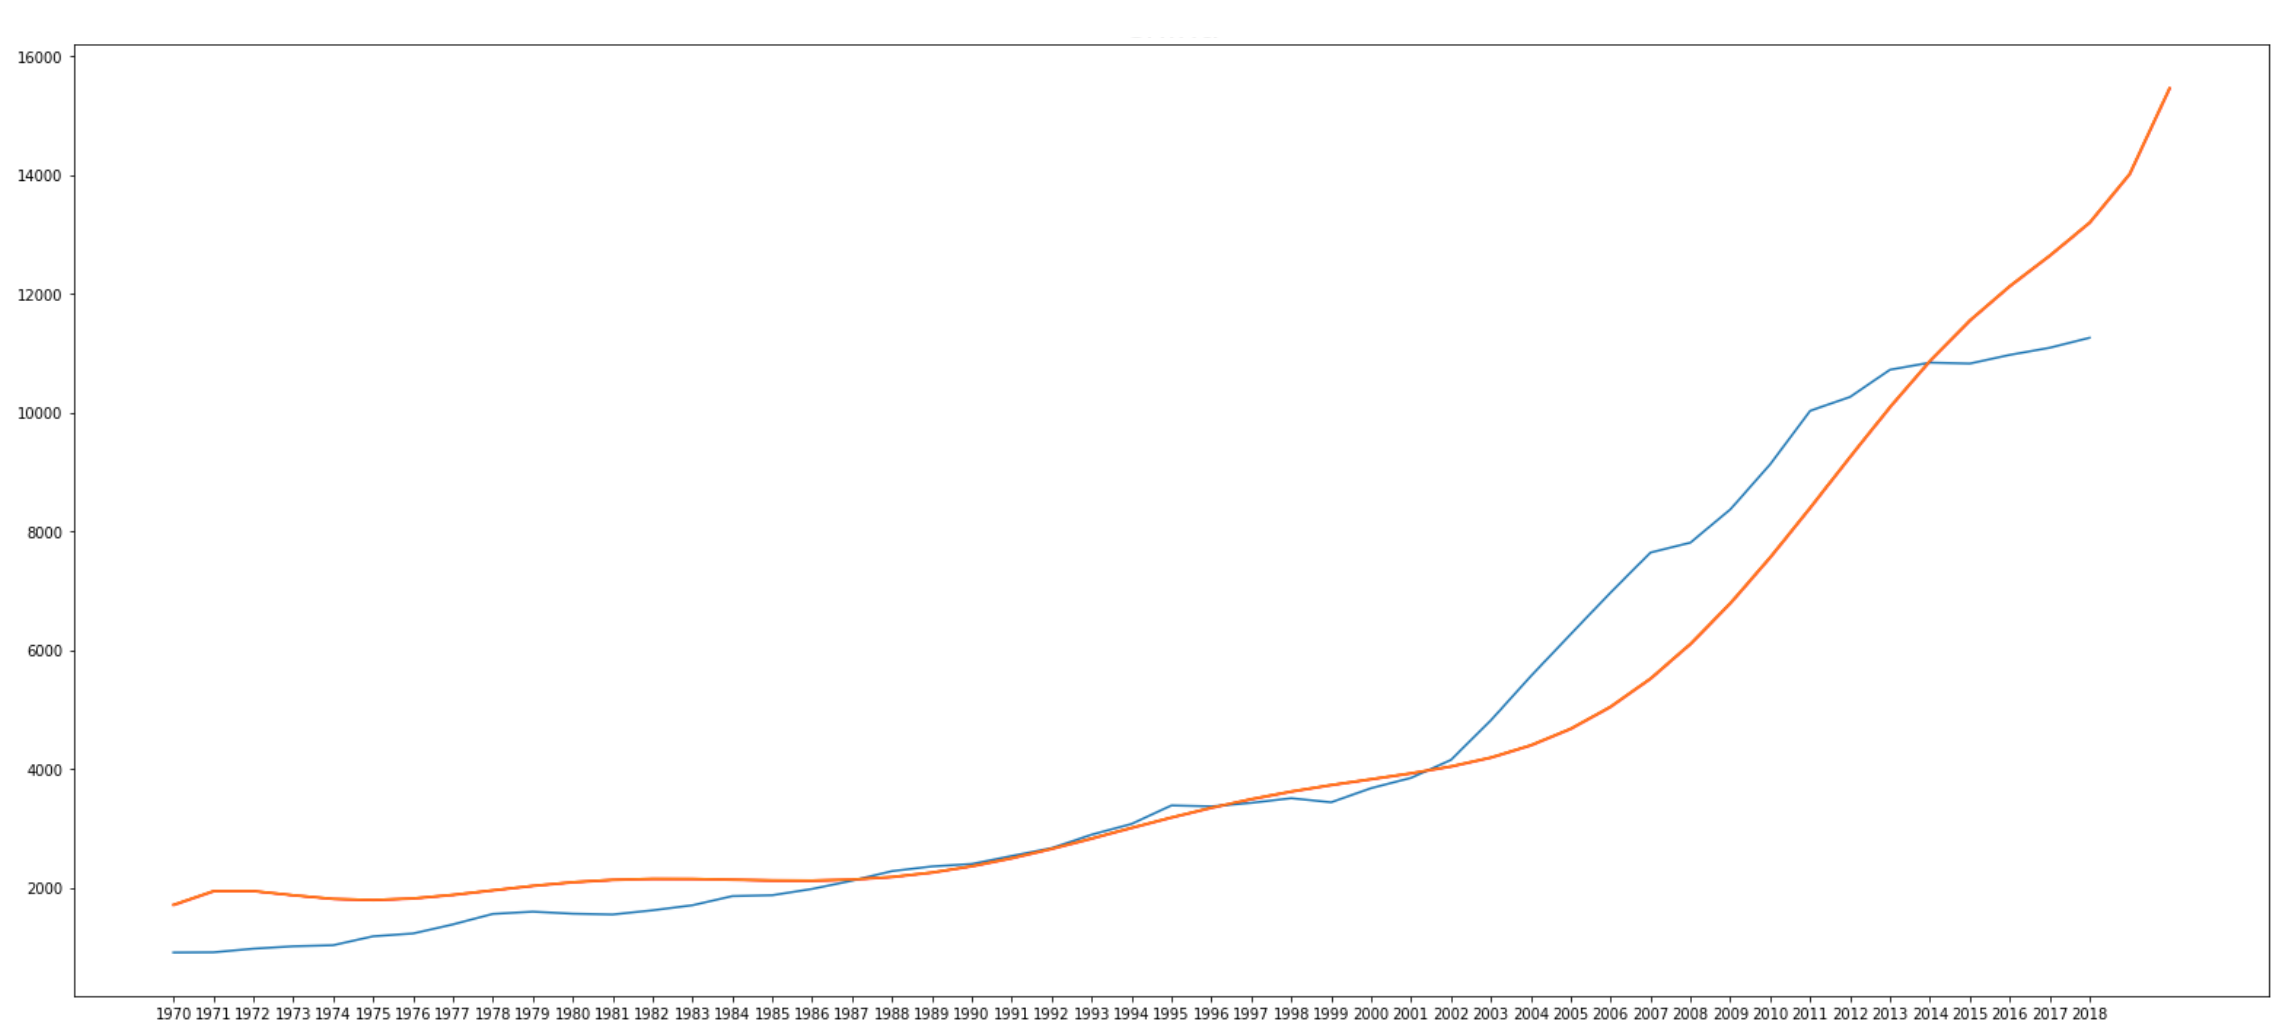
\includegraphics[width=0.5\linewidth]{ziedPNGS/4}}
	
	\subfloat[EU]{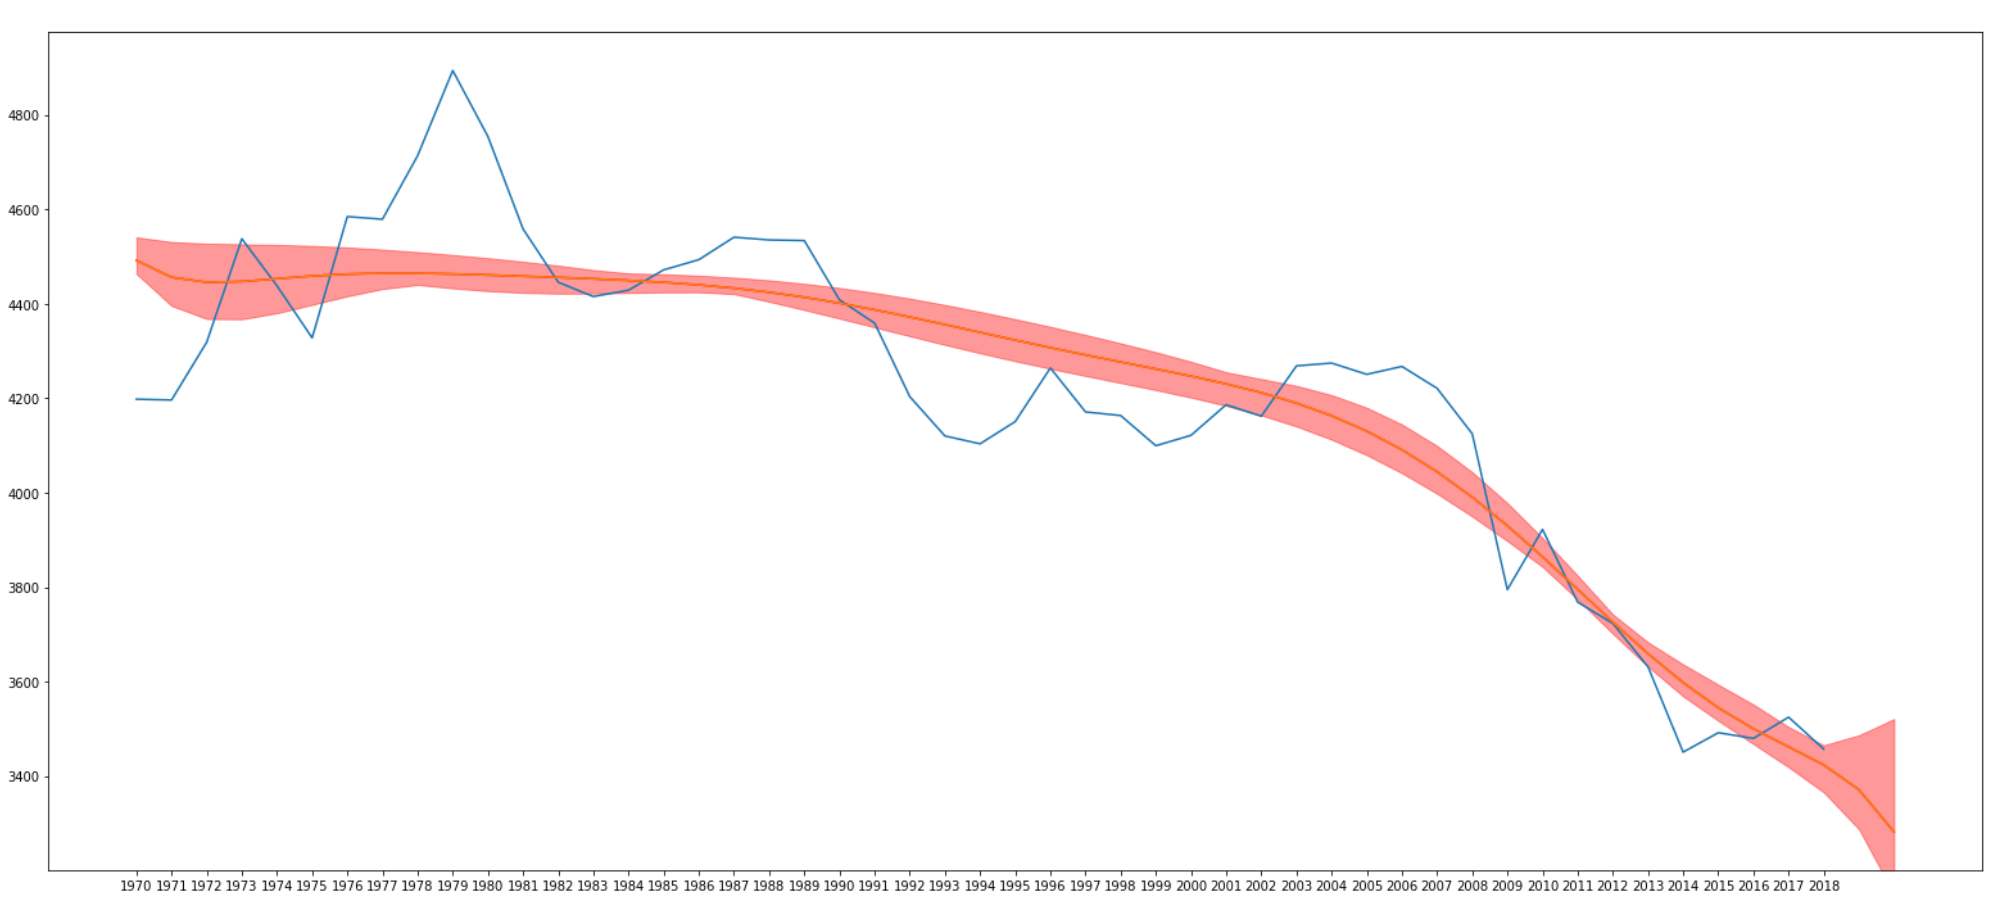
\includegraphics[width=0.5\linewidth]{ziedPNGS/5}}
	\subfloat[United States]{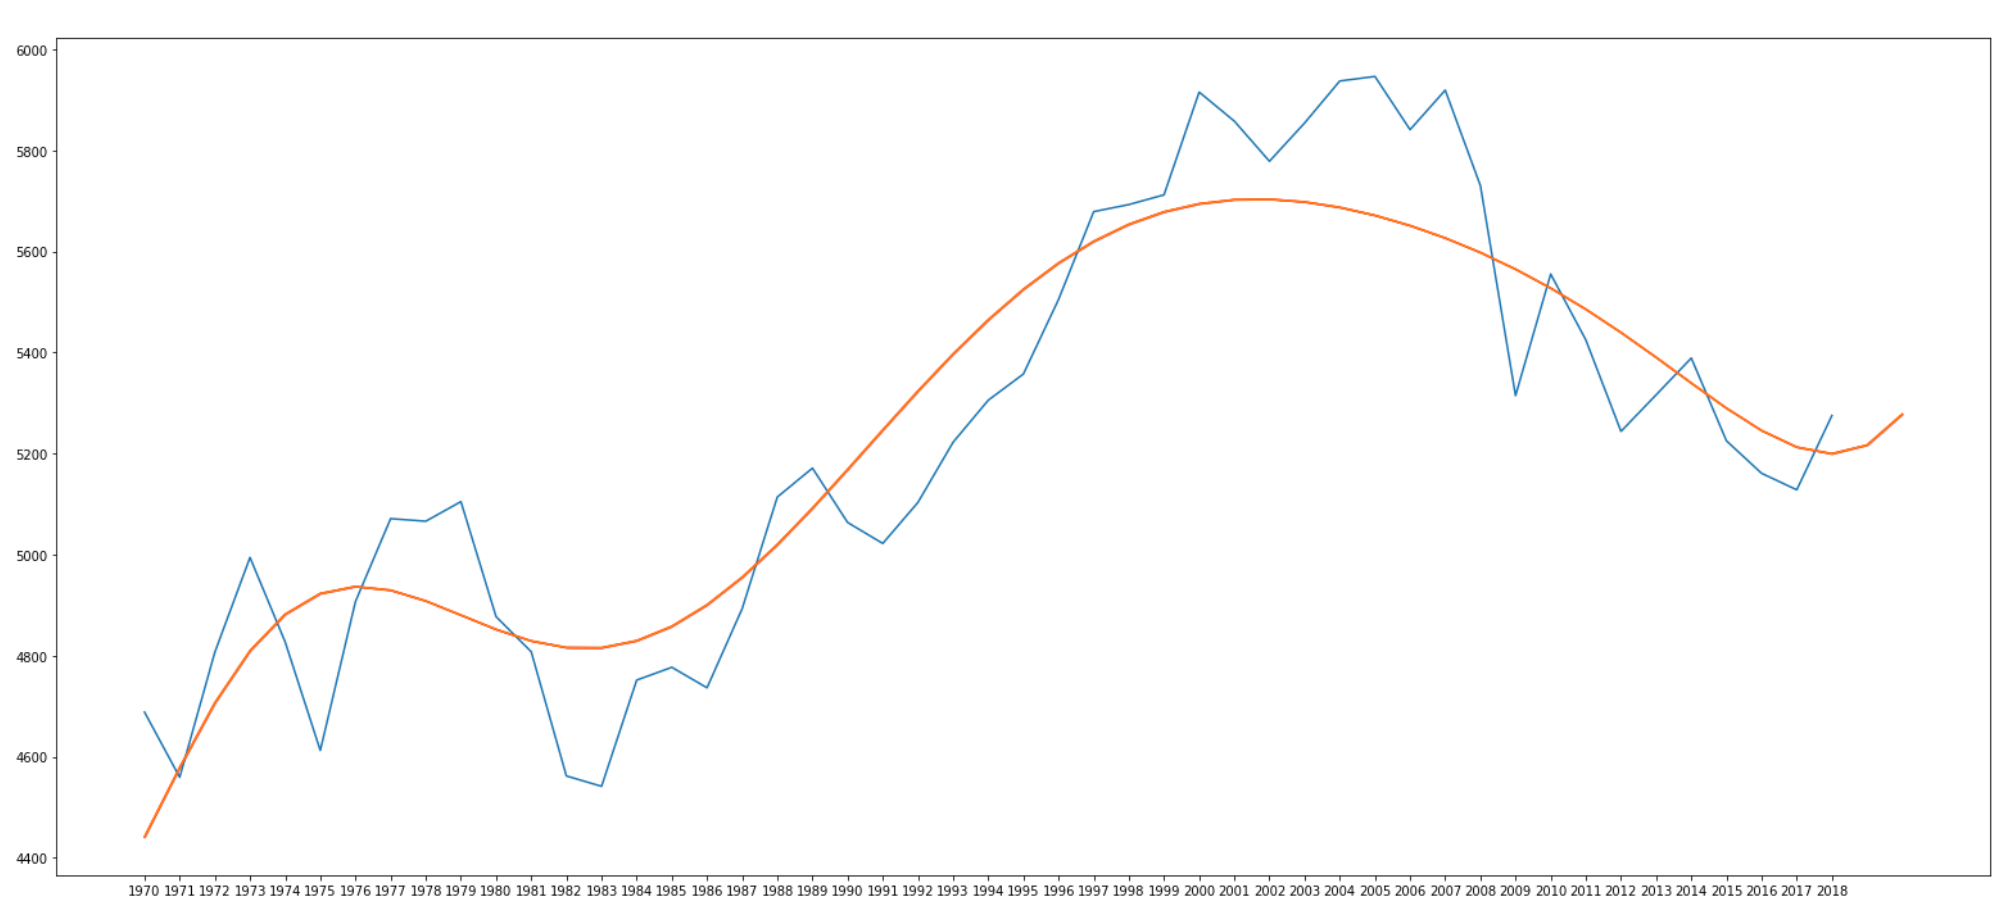
\includegraphics[width=0.5\linewidth]{ziedPNGS/6}}
	
	\subfloat[India]{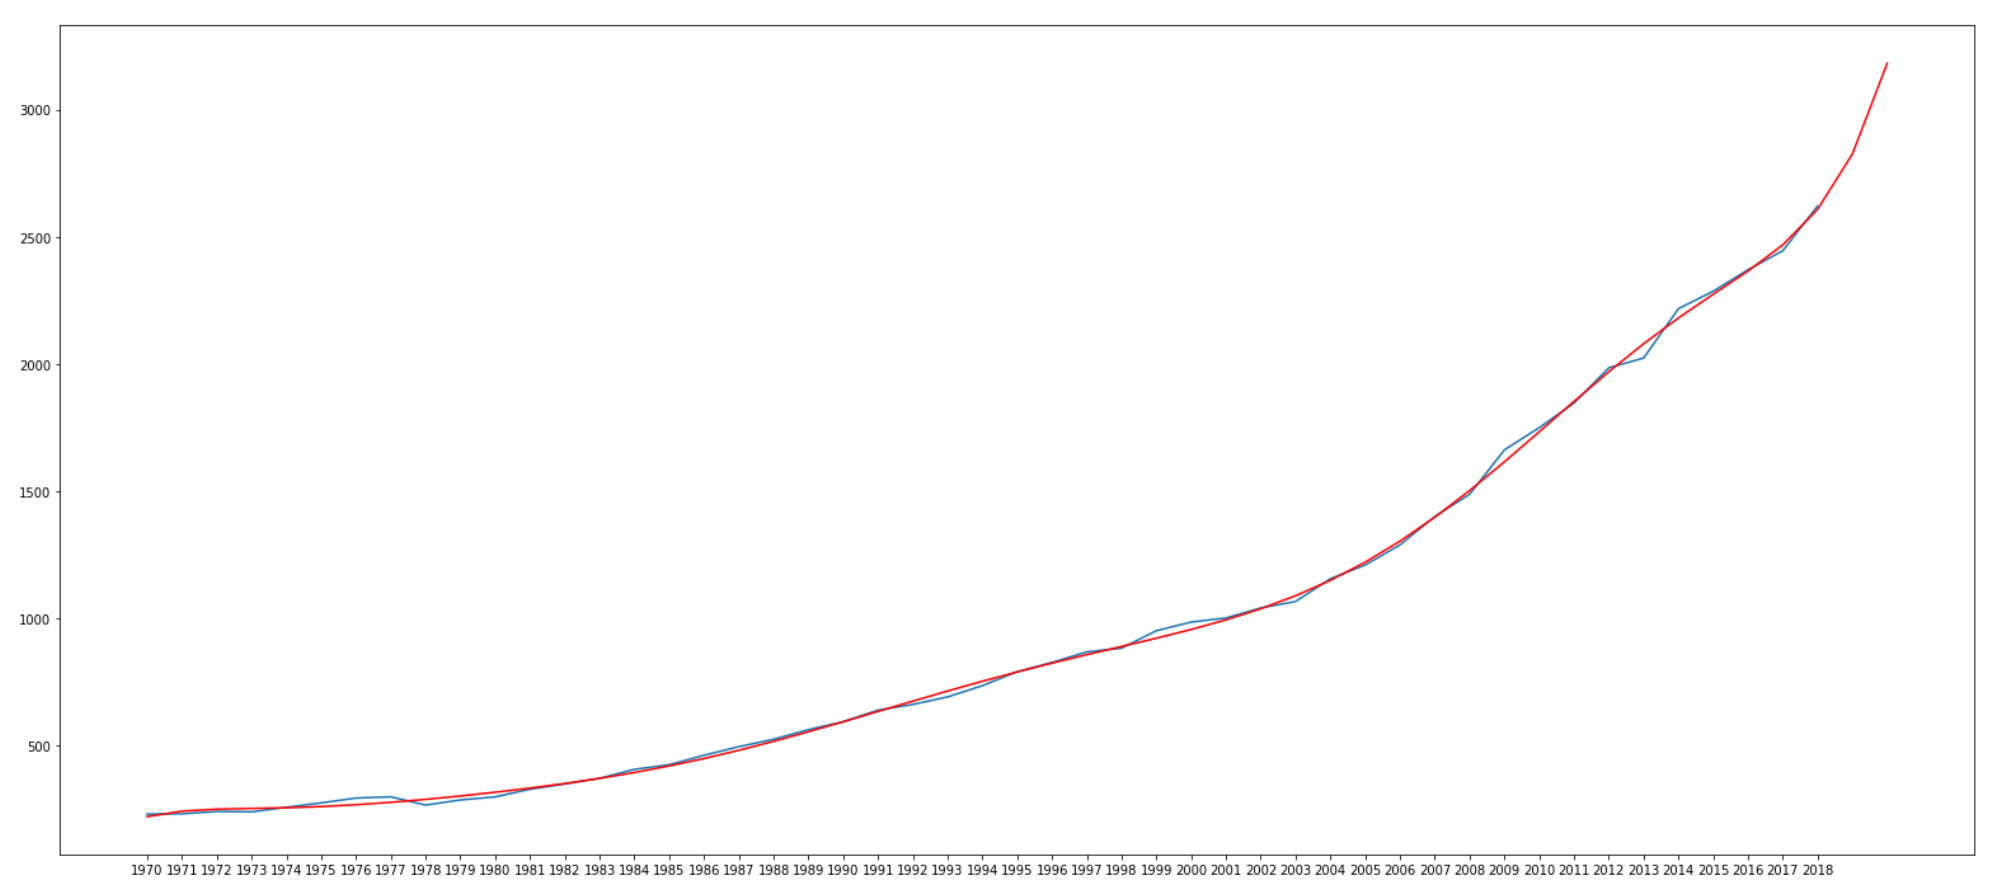
\includegraphics[width=0.5\linewidth]{ziedPNGS/7}}
	\caption{These graphs present the predicted emissions.}
	\label{fig:Results}
\end{figure}
